\documentclass[]{article}
\usepackage{lmodern}
\usepackage{amssymb,amsmath}
\usepackage{ifxetex,ifluatex}
\usepackage{fixltx2e} % provides \textsubscript
\ifnum 0\ifxetex 1\fi\ifluatex 1\fi=0 % if pdftex
  \usepackage[T1]{fontenc}
  \usepackage[utf8]{inputenc}
\else % if luatex or xelatex
  \ifxetex
    \usepackage{mathspec}
  \else
    \usepackage{fontspec}
  \fi
  \defaultfontfeatures{Ligatures=TeX,Scale=MatchLowercase}
\fi
% use upquote if available, for straight quotes in verbatim environments
\IfFileExists{upquote.sty}{\usepackage{upquote}}{}
% use microtype if available
\IfFileExists{microtype.sty}{%
\usepackage{microtype}
\UseMicrotypeSet[protrusion]{basicmath} % disable protrusion for tt fonts
}{}
\usepackage[margin=1in]{geometry}
\usepackage{hyperref}
\hypersetup{unicode=true,
            pdftitle={Renda per capita Metropolitana - Porto Alegre - RS},
            pdfauthor={Luciano Teixeira},
            pdfborder={0 0 0},
            breaklinks=true}
\urlstyle{same}  % don't use monospace font for urls
\usepackage{color}
\usepackage{fancyvrb}
\newcommand{\VerbBar}{|}
\newcommand{\VERB}{\Verb[commandchars=\\\{\}]}
\DefineVerbatimEnvironment{Highlighting}{Verbatim}{commandchars=\\\{\}}
% Add ',fontsize=\small' for more characters per line
\usepackage{framed}
\definecolor{shadecolor}{RGB}{248,248,248}
\newenvironment{Shaded}{\begin{snugshade}}{\end{snugshade}}
\newcommand{\KeywordTok}[1]{\textcolor[rgb]{0.13,0.29,0.53}{\textbf{#1}}}
\newcommand{\DataTypeTok}[1]{\textcolor[rgb]{0.13,0.29,0.53}{#1}}
\newcommand{\DecValTok}[1]{\textcolor[rgb]{0.00,0.00,0.81}{#1}}
\newcommand{\BaseNTok}[1]{\textcolor[rgb]{0.00,0.00,0.81}{#1}}
\newcommand{\FloatTok}[1]{\textcolor[rgb]{0.00,0.00,0.81}{#1}}
\newcommand{\ConstantTok}[1]{\textcolor[rgb]{0.00,0.00,0.00}{#1}}
\newcommand{\CharTok}[1]{\textcolor[rgb]{0.31,0.60,0.02}{#1}}
\newcommand{\SpecialCharTok}[1]{\textcolor[rgb]{0.00,0.00,0.00}{#1}}
\newcommand{\StringTok}[1]{\textcolor[rgb]{0.31,0.60,0.02}{#1}}
\newcommand{\VerbatimStringTok}[1]{\textcolor[rgb]{0.31,0.60,0.02}{#1}}
\newcommand{\SpecialStringTok}[1]{\textcolor[rgb]{0.31,0.60,0.02}{#1}}
\newcommand{\ImportTok}[1]{#1}
\newcommand{\CommentTok}[1]{\textcolor[rgb]{0.56,0.35,0.01}{\textit{#1}}}
\newcommand{\DocumentationTok}[1]{\textcolor[rgb]{0.56,0.35,0.01}{\textbf{\textit{#1}}}}
\newcommand{\AnnotationTok}[1]{\textcolor[rgb]{0.56,0.35,0.01}{\textbf{\textit{#1}}}}
\newcommand{\CommentVarTok}[1]{\textcolor[rgb]{0.56,0.35,0.01}{\textbf{\textit{#1}}}}
\newcommand{\OtherTok}[1]{\textcolor[rgb]{0.56,0.35,0.01}{#1}}
\newcommand{\FunctionTok}[1]{\textcolor[rgb]{0.00,0.00,0.00}{#1}}
\newcommand{\VariableTok}[1]{\textcolor[rgb]{0.00,0.00,0.00}{#1}}
\newcommand{\ControlFlowTok}[1]{\textcolor[rgb]{0.13,0.29,0.53}{\textbf{#1}}}
\newcommand{\OperatorTok}[1]{\textcolor[rgb]{0.81,0.36,0.00}{\textbf{#1}}}
\newcommand{\BuiltInTok}[1]{#1}
\newcommand{\ExtensionTok}[1]{#1}
\newcommand{\PreprocessorTok}[1]{\textcolor[rgb]{0.56,0.35,0.01}{\textit{#1}}}
\newcommand{\AttributeTok}[1]{\textcolor[rgb]{0.77,0.63,0.00}{#1}}
\newcommand{\RegionMarkerTok}[1]{#1}
\newcommand{\InformationTok}[1]{\textcolor[rgb]{0.56,0.35,0.01}{\textbf{\textit{#1}}}}
\newcommand{\WarningTok}[1]{\textcolor[rgb]{0.56,0.35,0.01}{\textbf{\textit{#1}}}}
\newcommand{\AlertTok}[1]{\textcolor[rgb]{0.94,0.16,0.16}{#1}}
\newcommand{\ErrorTok}[1]{\textcolor[rgb]{0.64,0.00,0.00}{\textbf{#1}}}
\newcommand{\NormalTok}[1]{#1}
\usepackage{graphicx,grffile}
\makeatletter
\def\maxwidth{\ifdim\Gin@nat@width>\linewidth\linewidth\else\Gin@nat@width\fi}
\def\maxheight{\ifdim\Gin@nat@height>\textheight\textheight\else\Gin@nat@height\fi}
\makeatother
% Scale images if necessary, so that they will not overflow the page
% margins by default, and it is still possible to overwrite the defaults
% using explicit options in \includegraphics[width, height, ...]{}
\setkeys{Gin}{width=\maxwidth,height=\maxheight,keepaspectratio}
\IfFileExists{parskip.sty}{%
\usepackage{parskip}
}{% else
\setlength{\parindent}{0pt}
\setlength{\parskip}{6pt plus 2pt minus 1pt}
}
\setlength{\emergencystretch}{3em}  % prevent overfull lines
\providecommand{\tightlist}{%
  \setlength{\itemsep}{0pt}\setlength{\parskip}{0pt}}
\setcounter{secnumdepth}{5}
% Redefines (sub)paragraphs to behave more like sections
\ifx\paragraph\undefined\else
\let\oldparagraph\paragraph
\renewcommand{\paragraph}[1]{\oldparagraph{#1}\mbox{}}
\fi
\ifx\subparagraph\undefined\else
\let\oldsubparagraph\subparagraph
\renewcommand{\subparagraph}[1]{\oldsubparagraph{#1}\mbox{}}
\fi

%%% Use protect on footnotes to avoid problems with footnotes in titles
\let\rmarkdownfootnote\footnote%
\def\footnote{\protect\rmarkdownfootnote}

%%% Change title format to be more compact
\usepackage{titling}

% Create subtitle command for use in maketitle
\newcommand{\subtitle}[1]{
  \posttitle{
    \begin{center}\large#1\end{center}
    }
}

\setlength{\droptitle}{-2em}

  \title{Renda per capita Metropolitana - Porto Alegre - RS}
    \pretitle{\vspace{\droptitle}\centering\huge}
  \posttitle{\par}
  \subtitle{Pós-Graduação Lato Senso - Big Data, Data Science e Data Analytics}
  \author{Luciano Teixeira}
    \preauthor{\centering\large\emph}
  \postauthor{\par}
      \predate{\centering\large\emph}
  \postdate{\par}
    \date{08/julho/2018}


\begin{document}
\maketitle

{
\setcounter{tocdepth}{2}
\tableofcontents
}
\section{Introdução da Análise}\label{introducao-da-analise}

O arquivo utilizado, se refere aos dados municipais do Atlas do
desenvolvimento humano no Brasil referentes aos Censos de 1991, 2000 e
2010 em \url{http://www.atlasbrasil.org.br/2013/pt/download/}.

Foram escolhidas 5 variáveis explicativas para a renda per capita dos
municípios.

\begin{verbatim}
* IDHM: Índice de Desenvolvimento Humano Municipal
* ESPVIDA:  Esperança de vida ao nascer
* GINI: Índice de Gini
* PESOURB:  População residente na área urbana
* T_FBSUPER:  Taxa de frequência bruta ao ensino superior
\end{verbatim}

A amostra será demonstrada por meio de uma análise descritiva des
variáveis explicaivas em relação à evolução da renda per capita dos
municípios da região metropolitana de Porto Alegre sobre os anos de
1991, 2000 e 2010.

Como método de análise, será utilizado regressão linear múltipla onde a
VR é a renda per capita e as variáveis explicativas são as 5 escolhidas
no passo 2.

\section{Inicializando Bibliotecas}\label{inicializando-bibliotecas}

Como primeiro passo, serão carregadas a seguintes bibliotecas. Caso
estas não se encontrem instaladas, é necessário que esta instalação seja
eetuada.

\begin{Shaded}
\begin{Highlighting}[]
\KeywordTok{library}\NormalTok{(readr)}
\KeywordTok{library}\NormalTok{(dplyr)}
\end{Highlighting}
\end{Shaded}

\begin{verbatim}
## 
## Attaching package: 'dplyr'
\end{verbatim}

\begin{verbatim}
## The following objects are masked from 'package:stats':
## 
##     filter, lag
\end{verbatim}

\begin{verbatim}
## The following objects are masked from 'package:base':
## 
##     intersect, setdiff, setequal, union
\end{verbatim}

\begin{Shaded}
\begin{Highlighting}[]
\KeywordTok{library}\NormalTok{(readxl)}
\KeywordTok{library}\NormalTok{(ggplot2)}
\KeywordTok{library}\NormalTok{(stringi)}
\KeywordTok{library}\NormalTok{(stringr)}
\KeywordTok{library}\NormalTok{(car)}
\end{Highlighting}
\end{Shaded}

\begin{verbatim}
## Loading required package: carData
\end{verbatim}

\begin{verbatim}
## 
## Attaching package: 'car'
\end{verbatim}

\begin{verbatim}
## The following object is masked from 'package:dplyr':
## 
##     recode
\end{verbatim}

\section{Importando Dados Brutos}\label{importando-dados-brutos}

\begin{Shaded}
\begin{Highlighting}[]
\NormalTok{dadosbrutos <-}\StringTok{ }\KeywordTok{read_excel}\NormalTok{(}\StringTok{"atlas2013_municipios.xlsx"}\NormalTok{)}
\end{Highlighting}
\end{Shaded}

\section{Especificando os Dados}\label{especificando-os-dados}

Comandos Encadeados podem demonstrar um principio de Machine Learning,
segregando cidades, Estado e Região. No caso deste modelo, oi delimitado
a Região Metropolitana de Porto Alegre, podendo ser aplicado em qualquer
estado, macro região ou micro região, com pequenos ajustes.

Este encadeameno de funçoes, substiui uma série de passos, utilizados
anteriormente para chegar à um resultado muito mais enchuto, levando em
consideração proficionais de analise de dados com poucos recursos em
questão de equipamenos, como por exemplos computadores de pequeno porte,
pouca memória e processador limitado.

\subsection{Dados de 2000}\label{dados-de-2000}

\begin{Shaded}
\begin{Highlighting}[]
\NormalTok{dadosrs <-}
\StringTok{  }\KeywordTok{filter}\NormalTok{(}
    \KeywordTok{select}\NormalTok{(}
      \KeywordTok{subset.data.frame}\NormalTok{(dadosbrutos, UF }\OperatorTok{==}\StringTok{ }\DecValTok{43}\NormalTok{),}
\NormalTok{      ANO,}
\NormalTok{      UF,}
\NormalTok{      MUNICIPIO,}
\NormalTok{      RDPC,}
\NormalTok{      IDHM,}
\NormalTok{      ESPVIDA,}
\NormalTok{      GINI,}
\NormalTok{      PESOURB,}
\NormalTok{      T_FBSUPER}
\NormalTok{    ),}
\NormalTok{    MUNICIPIO }\OperatorTok\StringTok{ }\KeywordTok{c}\NormalTok{(}\StringTok{"VIAMÃO"}\NormalTok{,}\StringTok{"TRIUNFO"}\NormalTok{,}\StringTok{"TAQUARA"}\NormalTok{,}\StringTok{"LEOPOLDO"}\NormalTok{,}\StringTok{"SÃO JERÔNIMO"}\NormalTok{,}
                     \StringTok{"SAPUCAIA DO SUL"}\NormalTok{,}\StringTok{"SAPIRANGA"}\NormalTok{,}\StringTok{"SANTO ANTÔNIO DA PATRULHA"}\NormalTok{,}
                     \StringTok{"PORTÃO"}\NormalTok{,}\StringTok{"PORTO ALEGRE"}\NormalTok{,}\StringTok{"PAROBÉ"}\NormalTok{,}\StringTok{"HAMBURGO"}\NormalTok{,}\StringTok{"NOVA SANTA RITA"}\NormalTok{,}
                     \StringTok{"NOVA HARTZ"}\NormalTok{,}\StringTok{"MONTENEGRO"}\NormalTok{,}\StringTok{"IVOTI"}\NormalTok{,}\StringTok{"GUAÍBA"}\NormalTok{,}\StringTok{"GRAVATAÍ"}\NormalTok{,}\StringTok{"GLORINHA"}\NormalTok{,}
                     \StringTok{"ESTÂNCIA VELHA"}\NormalTok{,}\StringTok{"ESTEIO"}\NormalTok{,}\StringTok{"ELDORADO DO SUL"}\NormalTok{,}\StringTok{"DOIS IRMÃOS"}\NormalTok{,}
                     \StringTok{"CHARQUEADAS"}\NormalTok{,}\StringTok{"CAPELA DE SANTANA"}\NormalTok{,}\StringTok{"CANOAS"}\NormalTok{,}\StringTok{"CAMPO BOM"}\NormalTok{,}
                     \StringTok{"CACHOEIRINHA"}\NormalTok{,}\StringTok{"ARROIO DOS RATOS"}\NormalTok{,}\StringTok{"ARARICÁ"}\NormalTok{,}\StringTok{"ALVORADA"}\NormalTok{),}
\NormalTok{    ANO }\OperatorTok{==}\StringTok{ }\DecValTok{2000}
\NormalTok{  )}
\end{Highlighting}
\end{Shaded}

\subsection{Listando os Dados de 2000}\label{listando-os-dados-de-2000}

\begin{Shaded}
\begin{Highlighting}[]
\KeywordTok{head}\NormalTok{(dadosrs)}
\end{Highlighting}
\end{Shaded}

\begin{verbatim}
## # A tibble: 6 x 9
##     ANO    UF MUNICIPIO         RDPC  IDHM ESPVIDA  GINI PESOURB T_FBSUPER
##   <dbl> <dbl> <chr>            <dbl> <dbl>   <dbl> <dbl>   <dbl>     <dbl>
## 1  2000    43 ALVORADA          429. 0.582    73.3  0.44  183365      6.71
## 2  2000    43 ARARICÁ           422. 0.565    71.3  0.42    3493      3.76
## 3  2000    43 ARROIO DOS RATOS  444. 0.61     71.4  0.5    12528     15.0 
## 4  2000    43 CACHOEIRINHA      629. 0.672    74.2  0.47  107564     15.7 
## 5  2000    43 CAMPO BOM         726. 0.669    74.1  0.48   51838     18.1 
## 6  2000    43 CANOAS            704. 0.665    74.1  0.52  306093     22.8
\end{verbatim}

Total de 29 registros.

\subsection{Sumário do Dados de 2000}\label{sumario-do-dados-de-2000}

\begin{Shaded}
\begin{Highlighting}[]
\KeywordTok{summary}\NormalTok{(dadosrs)}
\end{Highlighting}
\end{Shaded}

\begin{verbatim}
##       ANO             UF      MUNICIPIO              RDPC       
##  Min.   :2000   Min.   :43   Length:29          Min.   : 376.3  
##  1st Qu.:2000   1st Qu.:43   Class :character   1st Qu.: 504.5  
##  Median :2000   Median :43   Mode  :character   Median : 575.1  
##  Mean   :2000   Mean   :43                      Mean   : 600.1  
##  3rd Qu.:2000   3rd Qu.:43                      3rd Qu.: 670.7  
##  Max.   :2000   Max.   :43                      Max.   :1399.5  
##       IDHM           ESPVIDA           GINI           PESOURB       
##  Min.   :0.5340   Min.   :70.20   Min.   :0.3700   Min.   :   1285  
##  1st Qu.:0.6090   1st Qu.:72.06   1st Qu.:0.4500   1st Qu.:  13785  
##  Median :0.6280   Median :73.45   Median :0.4800   Median :  34367  
##  Mean   :0.6339   Mean   :73.26   Mean   :0.4862   Mean   : 107818  
##  3rd Qu.:0.6680   3rd Qu.:74.25   3rd Qu.:0.5200   3rd Qu.:  91956  
##  Max.   :0.7440   Max.   :76.11   Max.   :0.6100   Max.   :1320739  
##    T_FBSUPER    
##  Min.   : 3.76  
##  1st Qu.:11.16  
##  Median :14.25  
##  Mean   :15.55  
##  3rd Qu.:18.08  
##  Max.   :42.01
\end{verbatim}

\subsection{Dados de 2010}\label{dados-de-2010}

\begin{Shaded}
\begin{Highlighting}[]
\NormalTok{dadosrs_}\DecValTok{2010}\NormalTok{ <-}
\StringTok{  }\KeywordTok{filter}\NormalTok{(}
    \KeywordTok{select}\NormalTok{(}
      \KeywordTok{subset.data.frame}\NormalTok{(dadosbrutos, UF }\OperatorTok{==}\StringTok{ }\DecValTok{43}\NormalTok{),}
\NormalTok{      ANO,}
\NormalTok{      UF,}
\NormalTok{      MUNICIPIO,}
\NormalTok{      RDPC,}
\NormalTok{      IDHM,}
\NormalTok{      ESPVIDA,}
\NormalTok{      GINI,}
\NormalTok{      PESOURB,}
\NormalTok{      T_FBSUPER}
\NormalTok{    ),}
\NormalTok{    MUNICIPIO }\OperatorTok\StringTok{ }\KeywordTok{c}\NormalTok{(}\StringTok{"VIAMÃO"}\NormalTok{,}\StringTok{"TRIUNFO"}\NormalTok{,}\StringTok{"TAQUARA"}\NormalTok{,}\StringTok{"LEOPOLDO"}\NormalTok{,}\StringTok{"SÃO JERÔNIMO"}\NormalTok{,}
                     \StringTok{"SAPUCAIA DO SUL"}\NormalTok{,}\StringTok{"SAPIRANGA"}\NormalTok{,}\StringTok{"SANTO ANTÔNIO DA PATRULHA"}\NormalTok{,}
                     \StringTok{"PORTÃO"}\NormalTok{,}\StringTok{"PORTO ALEGRE"}\NormalTok{,}\StringTok{"PAROBÉ"}\NormalTok{,}\StringTok{"HAMBURGO"}\NormalTok{,}\StringTok{"NOVA SANTA RITA"}\NormalTok{,}
                     \StringTok{"NOVA HARTZ"}\NormalTok{,}\StringTok{"MONTENEGRO"}\NormalTok{,}\StringTok{"IVOTI"}\NormalTok{,}\StringTok{"GUAÍBA"}\NormalTok{,}\StringTok{"GRAVATAÍ"}\NormalTok{,}\StringTok{"GLORINHA"}\NormalTok{,}
                     \StringTok{"ESTÂNCIA VELHA"}\NormalTok{,}\StringTok{"ESTEIO"}\NormalTok{,}\StringTok{"ELDORADO DO SUL"}\NormalTok{,}\StringTok{"DOIS IRMÃOS"}\NormalTok{,}
                     \StringTok{"CHARQUEADAS"}\NormalTok{,}\StringTok{"CAPELA DE SANTANA"}\NormalTok{,}\StringTok{"CANOAS"}\NormalTok{,}\StringTok{"CAMPO BOM"}\NormalTok{,}
                     \StringTok{"CACHOEIRINHA"}\NormalTok{,}\StringTok{"ARROIO DOS RATOS"}\NormalTok{,}\StringTok{"ARARICÁ"}\NormalTok{,}\StringTok{"ALVORADA"}\NormalTok{),}
\NormalTok{    ANO }\OperatorTok{==}\StringTok{ }\DecValTok{2010}
\NormalTok{  )}
\end{Highlighting}
\end{Shaded}

\subsection{Listando os Dados de 2010}\label{listando-os-dados-de-2010}

\begin{Shaded}
\begin{Highlighting}[]
\KeywordTok{head}\NormalTok{(dadosrs_}\DecValTok{2010}\NormalTok{)}
\end{Highlighting}
\end{Shaded}

\begin{verbatim}
## # A tibble: 6 x 9
##     ANO    UF MUNICIPIO         RDPC  IDHM ESPVIDA  GINI PESOURB T_FBSUPER
##   <dbl> <dbl> <chr>            <dbl> <dbl>   <dbl> <dbl>   <dbl>     <dbl>
## 1  2010    43 ALVORADA          600. 0.699    77.4  0.43  195673      17.2
## 2  2010    43 ARARICÁ           610. 0.679    74.4  0.35    3996      15.4
## 3  2010    43 ARROIO DOS RATOS  624. 0.698    75.0  0.46   12956      27.2
## 4  2010    43 CACHOEIRINHA      844. 0.757    76.4  0.44  118278      37.7
## 5  2010    43 CAMPO BOM         880. 0.745    76.1  0.43   57338      29.0
## 6  2010    43 CANOAS            952. 0.75     76.8  0.51  323827      42
\end{verbatim}

Total de 29 registros.

\subsection{Sumário do Dados de 2010}\label{sumario-do-dados-de-2010}

\begin{Shaded}
\begin{Highlighting}[]
\KeywordTok{summary}\NormalTok{(dadosrs_}\DecValTok{2010}\NormalTok{)}
\end{Highlighting}
\end{Shaded}

\begin{verbatim}
##       ANO             UF      MUNICIPIO              RDPC       
##  Min.   :2010   Min.   :43   Length:29          Min.   : 533.9  
##  1st Qu.:2010   1st Qu.:43   Class :character   1st Qu.: 687.0  
##  Median :2010   Median :43   Mode  :character   Median : 733.3  
##  Mean   :2010   Mean   :43                      Mean   : 789.8  
##  3rd Qu.:2010   3rd Qu.:43                      3rd Qu.: 871.4  
##  Max.   :2010   Max.   :43                      Max.   :1758.3  
##       IDHM          ESPVIDA           GINI           PESOURB       
##  Min.   :0.661   Min.   :73.93   Min.   :0.3400   Min.   :   2067  
##  1st Qu.:0.711   1st Qu.:75.57   1st Qu.:0.4200   1st Qu.:  18062  
##  Median :0.726   Median :76.37   Median :0.4400   Median :  41484  
##  Mean   :0.727   Mean   :76.21   Mean   :0.4431   Mean   : 117138  
##  3rd Qu.:0.747   3rd Qu.:76.95   3rd Qu.:0.4700   3rd Qu.:  93064  
##  Max.   :0.805   Max.   :78.23   Max.   :0.6000   Max.   :1409351  
##    T_FBSUPER    
##  Min.   :15.42  
##  1st Qu.:24.41  
##  Median :28.99  
##  Mean   :30.84  
##  3rd Qu.:35.09  
##  Max.   :64.55
\end{verbatim}

\section{Segregando os Dados em Relação a Variavel Y =
RDPC}\label{segregando-os-dados-em-relacao-a-variavel-y-rdpc}

\begin{Shaded}
\begin{Highlighting}[]
\NormalTok{Y_RDPC_}\DecValTok{2010}\NormalTok{ <-}\StringTok{ }\KeywordTok{c}\NormalTok{(dadosrs_}\DecValTok{2010}\OperatorTok{$}\NormalTok{RDPC)}
\end{Highlighting}
\end{Shaded}

\section{Inserindo os dados de 2010 na base de
2000}\label{inserindo-os-dados-de-2010-na-base-de-2000}

\begin{Shaded}
\begin{Highlighting}[]
\NormalTok{dadosrs<-}\StringTok{ }\KeywordTok{data.frame}\NormalTok{(dadosrs,Y_RDPC_}\DecValTok{2010}\NormalTok{)}
\end{Highlighting}
\end{Shaded}

\section{Sumário de variáveis}\label{sumario-de-variaveis}

\begin{Shaded}
\begin{Highlighting}[]
\KeywordTok{summary}\NormalTok{(dadosrs)}
\end{Highlighting}
\end{Shaded}

\begin{verbatim}
##       ANO             UF      MUNICIPIO              RDPC       
##  Min.   :2000   Min.   :43   Length:29          Min.   : 376.3  
##  1st Qu.:2000   1st Qu.:43   Class :character   1st Qu.: 504.5  
##  Median :2000   Median :43   Mode  :character   Median : 575.1  
##  Mean   :2000   Mean   :43                      Mean   : 600.1  
##  3rd Qu.:2000   3rd Qu.:43                      3rd Qu.: 670.7  
##  Max.   :2000   Max.   :43                      Max.   :1399.5  
##       IDHM           ESPVIDA           GINI           PESOURB       
##  Min.   :0.5340   Min.   :70.20   Min.   :0.3700   Min.   :   1285  
##  1st Qu.:0.6090   1st Qu.:72.06   1st Qu.:0.4500   1st Qu.:  13785  
##  Median :0.6280   Median :73.45   Median :0.4800   Median :  34367  
##  Mean   :0.6339   Mean   :73.26   Mean   :0.4862   Mean   : 107818  
##  3rd Qu.:0.6680   3rd Qu.:74.25   3rd Qu.:0.5200   3rd Qu.:  91956  
##  Max.   :0.7440   Max.   :76.11   Max.   :0.6100   Max.   :1320739  
##    T_FBSUPER      Y_RDPC_2010    
##  Min.   : 3.76   Min.   : 533.9  
##  1st Qu.:11.16   1st Qu.: 687.0  
##  Median :14.25   Median : 733.3  
##  Mean   :15.55   Mean   : 789.8  
##  3rd Qu.:18.08   3rd Qu.: 871.4  
##  Max.   :42.01   Max.   :1758.3
\end{verbatim}

\section{Histogramas}\label{histogramas}

\begin{Shaded}
\begin{Highlighting}[]
\KeywordTok{par}\NormalTok{(}\DataTypeTok{mfrow =} \KeywordTok{c}\NormalTok{(}\DecValTok{2}\NormalTok{,}\DecValTok{2}\NormalTok{))}

\KeywordTok{hist}\NormalTok{(dadosrs}\OperatorTok{$}\NormalTok{RDPC, }\DataTypeTok{xlab =} \StringTok{"RDPC"}\NormalTok{, }\DataTypeTok{main =} \StringTok{"HIST RDPC"}\NormalTok{)}
\KeywordTok{hist}\NormalTok{(dadosrs}\OperatorTok{$}\NormalTok{IDHM, }\DataTypeTok{xlab =} \StringTok{"IDHM"}\NormalTok{, }\DataTypeTok{main =} \StringTok{"HIST IDHM"}\NormalTok{)}
\KeywordTok{hist}\NormalTok{(dadosrs}\OperatorTok{$}\NormalTok{GINI, }\DataTypeTok{xlab =} \StringTok{"GINI"}\NormalTok{, }\DataTypeTok{main =} \StringTok{"HIST GINI"}\NormalTok{)}
\KeywordTok{hist}\NormalTok{(dadosrs}\OperatorTok{$}\NormalTok{Y_RDPC_}\DecValTok{2010}\NormalTok{, }\DataTypeTok{xlab =} \StringTok{"RDPC"}\NormalTok{, }\DataTypeTok{main =} \StringTok{"HIST RDPC 2010"}\NormalTok{)}
\end{Highlighting}
\end{Shaded}

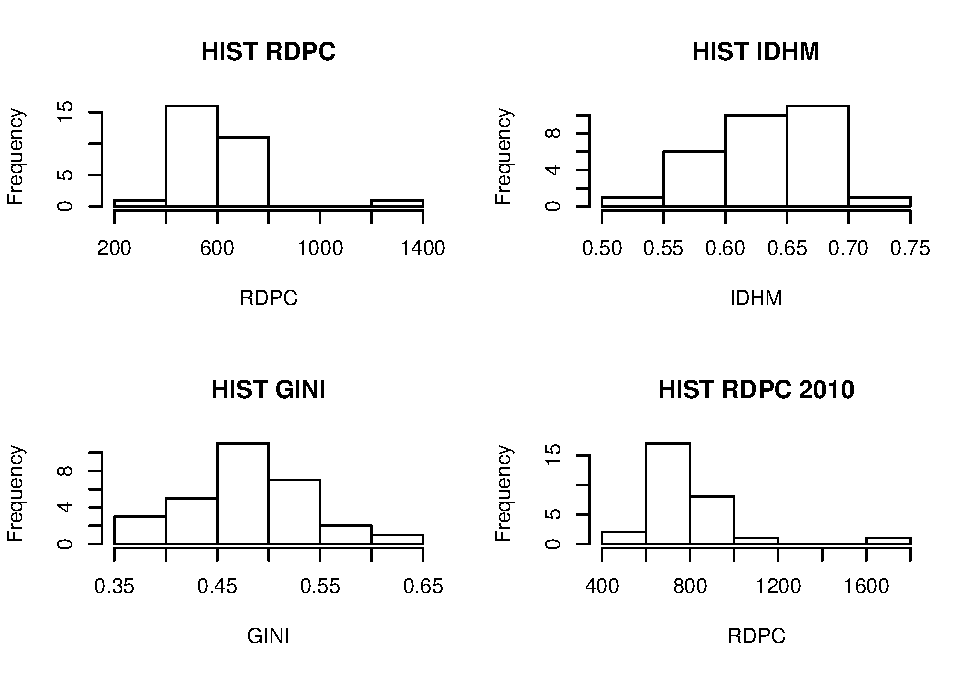
\includegraphics{AnaliseRegressaoRendaPerCaptaRS_files/figure-latex/histogramas-1.pdf}

\section{Análise de correlação linear entre duas variáveis
quantitativas}\label{analise-de-correlacao-linear-entre-duas-variaveis-quantitativas}

\begin{Shaded}
\begin{Highlighting}[]
\KeywordTok{plot}\NormalTok{(dadosrs}\OperatorTok{$}\NormalTok{GINI,dadosrs}\OperatorTok{$}\NormalTok{ESPVIDA)}
\end{Highlighting}
\end{Shaded}

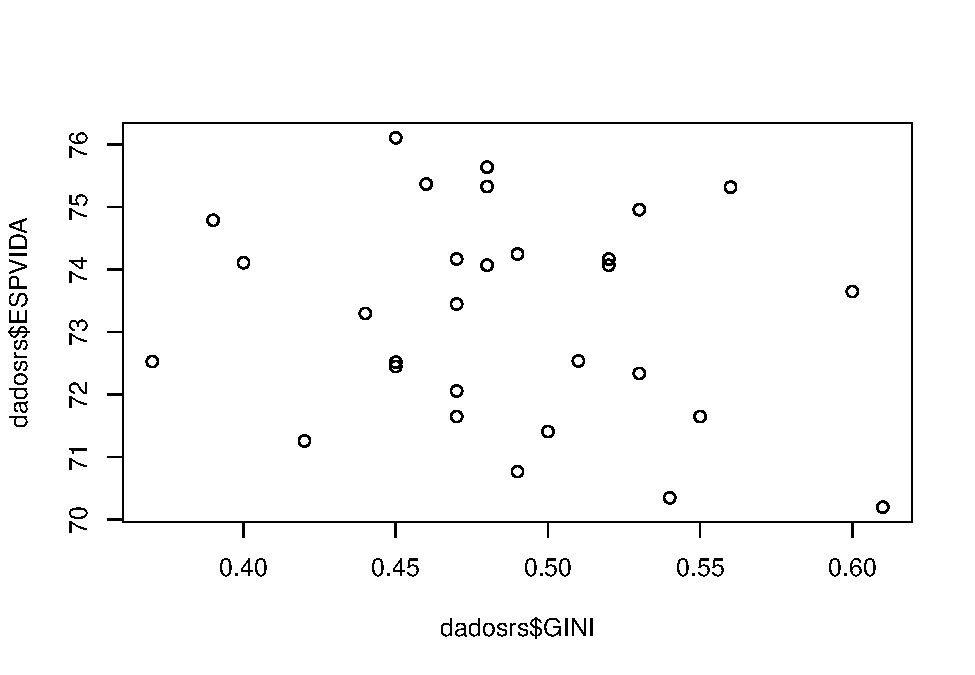
\includegraphics{AnaliseRegressaoRendaPerCaptaRS_files/figure-latex/correlacao_plot-1.pdf}

\begin{Shaded}
\begin{Highlighting}[]
\KeywordTok{cor}\NormalTok{(dadosrs}\OperatorTok{$}\NormalTok{GINI,dadosrs}\OperatorTok{$}\NormalTok{ESPVIDA)}
\end{Highlighting}
\end{Shaded}

\begin{verbatim}
## [1] -0.1923844
\end{verbatim}

\section{Aplicação da Regressao
Multipla}\label{aplicacao-da-regressao-multipla}

\begin{Shaded}
\begin{Highlighting}[]
\NormalTok{reg <-}\StringTok{ }\KeywordTok{lm}\NormalTok{(RDPC }\OperatorTok{~}\StringTok{ }\NormalTok{IDHM }\OperatorTok{+}\StringTok{ }\NormalTok{ESPVIDA }\OperatorTok{+}\StringTok{ }\NormalTok{GINI }\OperatorTok{+}\StringTok{ }\NormalTok{PESOURB }\OperatorTok{+}\StringTok{ }\NormalTok{T_FBSUPER, }\DataTypeTok{data =}\NormalTok{ dadosrs)}
\end{Highlighting}
\end{Shaded}

\section{Teste a significância global do modelo de
regressão.}\label{teste-a-significancia-global-do-modelo-de-regressao.}

\begin{Shaded}
\begin{Highlighting}[]
\KeywordTok{summary}\NormalTok{(reg)}
\end{Highlighting}
\end{Shaded}

\begin{verbatim}
## 
## Call:
## lm(formula = RDPC ~ IDHM + ESPVIDA + GINI + PESOURB + T_FBSUPER, 
##     data = dadosrs)
## 
## Residuals:
##      Min       1Q   Median       3Q      Max 
## -100.383  -42.143   -0.363   38.871   91.328 
## 
## Coefficients:
##               Estimate Std. Error t value Pr(>|t|)    
## (Intercept) -1.686e+02  5.908e+02  -0.285  0.77798    
## IDHM         1.004e+03  4.913e+02   2.043  0.05267 .  
## ESPVIDA     -1.204e+00  8.384e+00  -0.144  0.88709    
## GINI         4.911e+01  2.530e+02   0.194  0.84778    
## PESOURB      3.012e-04  5.657e-05   5.324  2.1e-05 ***
## T_FBSUPER    1.056e+01  3.138e+00   3.366  0.00267 ** 
## ---
## Signif. codes:  0 '***' 0.001 '**' 0.01 '*' 0.05 '.' 0.1 ' ' 1
## 
## Residual standard error: 56.03 on 23 degrees of freedom
## Multiple R-squared:  0.9255, Adjusted R-squared:  0.9093 
## F-statistic: 57.16 on 5 and 23 DF,  p-value: 3.287e-12
\end{verbatim}

\section{Intervalos de confiança para os coeficientes da
equação.}\label{intervalos-de-confianca-para-os-coeficientes-da-equacao.}

\begin{Shaded}
\begin{Highlighting}[]
\KeywordTok{confint}\NormalTok{(reg)}
\end{Highlighting}
\end{Shaded}

\begin{verbatim}
##                     2.5 %       97.5 %
## (Intercept) -1.390756e+03 1.053655e+03
## IDHM        -1.256329e+01 2.020167e+03
## ESPVIDA     -1.854803e+01 1.614057e+01
## GINI        -4.742425e+02 5.724709e+02
## PESOURB      1.841587e-04 4.182144e-04
## T_FBSUPER    4.071895e+00 1.705401e+01
\end{verbatim}

\section{Distribuição dos Resíduos}\label{distribuicao-dos-residuos}

\begin{Shaded}
\begin{Highlighting}[]
\KeywordTok{par}\NormalTok{(}\DataTypeTok{mfrow =} \KeywordTok{c}\NormalTok{(}\DecValTok{2}\NormalTok{,}\DecValTok{2}\NormalTok{))}

\KeywordTok{plot}\NormalTok{(}\KeywordTok{fitted}\NormalTok{(reg),}\KeywordTok{residuals}\NormalTok{(reg),}\DataTypeTok{xlab=}\StringTok{"Valores Ajustados"}\NormalTok{,}\DataTypeTok{ylab=}\StringTok{"Resíduos"}\NormalTok{)}
\KeywordTok{abline}\NormalTok{(}\DataTypeTok{h=}\DecValTok{0}\NormalTok{)}

\KeywordTok{plot}\NormalTok{(dadosrs}\OperatorTok{$}\NormalTok{GINI,}\KeywordTok{residuals}\NormalTok{(reg),}\DataTypeTok{xlab=}\StringTok{"GINI"}\NormalTok{,}\DataTypeTok{ylab=}\StringTok{"Resíduos"}\NormalTok{)}
\KeywordTok{abline}\NormalTok{(}\DataTypeTok{h=}\DecValTok{0}\NormalTok{)}

\KeywordTok{plot}\NormalTok{(dadosrs}\OperatorTok{$}\NormalTok{ESPVIDA,}\KeywordTok{residuals}\NormalTok{(reg),}\DataTypeTok{xlab=}\StringTok{"ESPVIDA"}\NormalTok{,}\DataTypeTok{ylab=}\StringTok{"Resíduos"}\NormalTok{)}
\KeywordTok{abline}\NormalTok{(}\DataTypeTok{h=}\DecValTok{0}\NormalTok{)}
\end{Highlighting}
\end{Shaded}

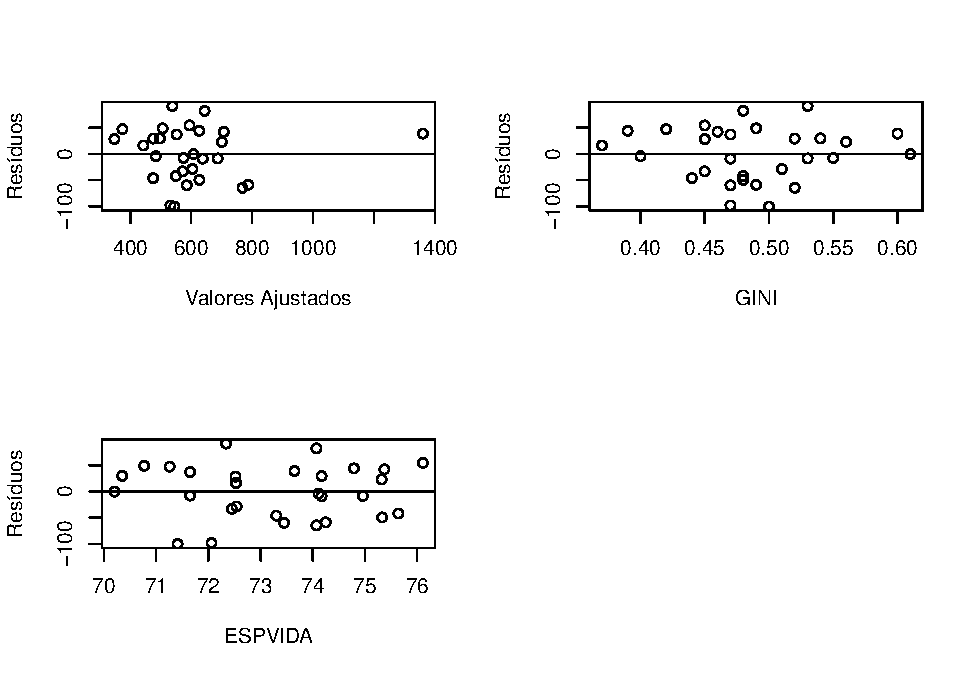
\includegraphics{AnaliseRegressaoRendaPerCaptaRS_files/figure-latex/residuos-1.pdf}

\section{Teste de Shapiro}\label{teste-de-shapiro}

\begin{Shaded}
\begin{Highlighting}[]
\KeywordTok{shapiro.test}\NormalTok{(reg}\OperatorTok{$}\NormalTok{residuals)}
\end{Highlighting}
\end{Shaded}

\begin{verbatim}
## 
##  Shapiro-Wilk normality test
## 
## data:  reg$residuals
## W = 0.96435, p-value = 0.4185
\end{verbatim}

\section{Outliers}\label{outliers}

Não foi detetado nenhum outliers.

\begin{Shaded}
\begin{Highlighting}[]
\KeywordTok{which}\NormalTok{(}\KeywordTok{rstudent}\NormalTok{(reg) }\OperatorTok{>}\StringTok{ }\DecValTok{2}\NormalTok{)}
\end{Highlighting}
\end{Shaded}

\begin{verbatim}
## 22 
## 22
\end{verbatim}

\section{Multicolinearidade}\label{multicolinearidade}

Multicolinearidade consiste em um problema comum em regressões, no qual
as variáveis independentes possuem relações lineares exatas ou
aproximadamente exatas.

\subsection{Multicolinearidade 01}\label{multicolinearidade-01}

\begin{Shaded}
\begin{Highlighting}[]
\KeywordTok{attach}\NormalTok{(dadosrs)}
\end{Highlighting}
\end{Shaded}

\begin{verbatim}
## The following object is masked _by_ .GlobalEnv:
## 
##     Y_RDPC_2010
\end{verbatim}

\begin{Shaded}
\begin{Highlighting}[]
\KeywordTok{pairs}\NormalTok{(dadosrs[,}\KeywordTok{c}\NormalTok{(}\DecValTok{4}\OperatorTok{:}\DecValTok{10}\NormalTok{)])}
\end{Highlighting}
\end{Shaded}

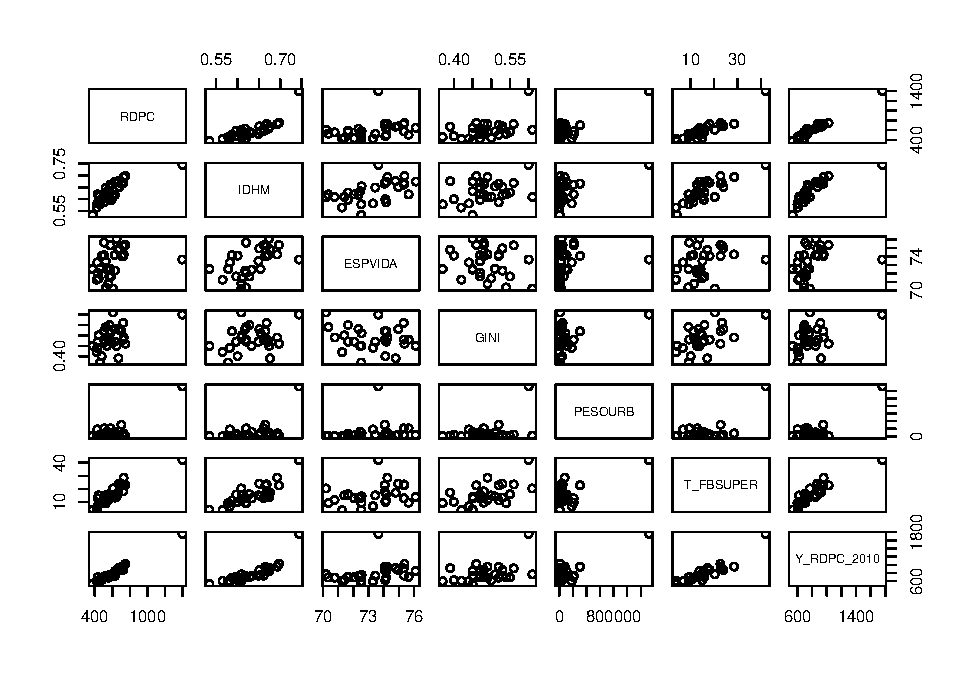
\includegraphics{AnaliseRegressaoRendaPerCaptaRS_files/figure-latex/multicolinearidade01-1.pdf}

\begin{Shaded}
\begin{Highlighting}[]
\KeywordTok{round}\NormalTok{(}\KeywordTok{cor}\NormalTok{(dadosrs[,}\KeywordTok{c}\NormalTok{(}\DecValTok{4}\OperatorTok{:}\DecValTok{10}\NormalTok{)]),}\DecValTok{3}\NormalTok{)}
\end{Highlighting}
\end{Shaded}

\begin{verbatim}
##              RDPC  IDHM ESPVIDA   GINI PESOURB T_FBSUPER Y_RDPC_2010
## RDPC        1.000 0.812   0.305  0.492   0.811     0.906       0.983
## IDHM        0.812 1.000   0.527  0.322   0.512     0.824       0.833
## ESPVIDA     0.305 0.527   1.000 -0.192   0.157     0.287       0.345
## GINI        0.492 0.322  -0.192  1.000   0.371     0.562       0.439
## PESOURB     0.811 0.512   0.157  0.371   1.000     0.645       0.826
## T_FBSUPER   0.906 0.824   0.287  0.562   0.645     1.000       0.905
## Y_RDPC_2010 0.983 0.833   0.345  0.439   0.826     0.905       1.000
\end{verbatim}

\subsection{Multicolinearidade 02}\label{multicolinearidade-02}

Foram detetados valores superiores a 5, que indicam associação muito
fraca entre variáveis explicativas.

\begin{Shaded}
\begin{Highlighting}[]
\KeywordTok{vif}\NormalTok{(reg)}
\end{Highlighting}
\end{Shaded}

\begin{verbatim}
##      IDHM   ESPVIDA      GINI   PESOURB T_FBSUPER 
##  4.411788  1.747208  1.836354  1.716155  5.346944
\end{verbatim}


\end{document}
